\chapter{Differenze tra Initial Coin Offering e Security Token Offering}                %crea il capitolo
%%%%%%%%%%%%%%%%%%%%%%%%%%%%%%%%%%%%%%%%%imposta l'intestazione di pagina
\lhead[\fancyplain{}{\bfseries\thepage}]{\fancyplain{}{\bfseries\rightmark}}
\pagenumbering{arabic}
%mette i numeri arabi


\section{Breve storia delle monete elettroniche e delle cryptocurrency}

Sebbene le valute digitali abbiano raggiunto un nuovo livello di rilievo nel mondo solo negli ultimi anni, è importante ricordare che la monete elletroniche hanno una storia che risale a decenni fa. Il white paper “Bitcoin: A Peer-to-Peer Electronic Cash System”, pubblicato nel 2008 da un autore anonimo o da un gruppo di persone sotto lo pseudonimo di Satoshi Nakamoto, per quanto risulti innovativo e a posteriori anche rivoluzionario, si basa su tecnologie preesistenti e ben affermate tra le quali ad esempio le reti P2P, un fenomeno che ha radici nelle prime fasi della storia di Internet e reso popolare da Napster. Non sono solo le reti distribuite ad essere una fondazione per Bitcoin; nel white paper Nakamoto si avvale infatti di altri lavori precedenti che risultano fondamentali al funzionamento della rete. Tra questi possiamo citare il lavoro di tesi pubblicato da Ralph Merkle nei primi anni ’70  riguardo alla comunicazione sicura attraverso canali insicuri e gli sviluppi apportati da Diffie e Hellman. Inoltre, è proprio a Merkle che dobbiamo l’invenzione dei Merkle Tree usati in Bitcoin poiché forniscono un metodo per firmare digitalmente messaggi contenuti in grandi strutture dati. I merklee tree verrano successivamente ripresi da Bayer, Haber e Stornetta per la realizzazione efficiente di una catena di blocchi firmata crittograficamente.


Altri lavori più recenti risultano essere punti chiave per lo sviluppo della rete Bitcoin ed in generale dei sistemi di pagamento elettronici.


Nel 1983 in “Blind Signatures for Untraceable Payments” e nei sui lavori successivi, Chaum introduce l’idea di un sistema di pagamento elettronico anonimo basato sulla tecnologia di Blind Signature, sistema che verrà poi implementato dallo stesso autore con ECash™ nel 1994. Come osserva Schoenmakers nonostante le istituzioni finanziare già utilizzassero dietro le quinte sistemi elettronici per processare transazioni l’apertura al pubblico dei sistemi di pagamento elettronici introduce la necessità di un sistema di pagamento elettronico che possa essere utilizzato in una rete ad accesso pubblico, particolarmente in riferimento alla rete Internet. Nel 1998 DigiCash fallisce, principalmente a causa della forte competizione posta in atto dal sistema di pagamento tramite carta di credito. Nel particolare secondo Chaum la compagnia ha sofferto di un chicken-and-egg problem: fu difficile convincere abbastanza venditori  ad adottare il sistema per  poter acquisire clienti e vice versa. (Lo stesso destino spetta ad altre forme di pagamento elettronico dello stesso periodo tra le quali possono essere citate CyberCoin, Virtual PIN. ) 


Sebbene infruttuosa, l’esperienza di Chaum rappresenta il primo esempio di un sistema di pagamento elettronico anonimo e risulta pioneristico sia nei problemi che vengono presentati come nelle soluzioni proposte a quest’ultimi, come avviene nel caso del problema di double spending. 


Altri sistemi di moneta digitale si sono susseguiti negli anni, tra i più rilevanti possiamo citare e-gold, Liberty Reserve e PayPal: I primi due non più attivi, entrambi per controversie legali, mentre l’ultimo ancora attivo. Questa lista non ha scopo di essere esauriente, per un approfondimento si rimanda alla letteratura sull’argomento.
Un altro tassello fondamentale nello sviluppo delle monete elettroniche è l’introduzione nel 1997 di hashcash da parte di Adam Back che indipendentemente descrive un sistema simile a quanto proposto da Cynthia Dwork,  Moni Naor e Eli Ponyatovski nel 1992 in “Pricing via Processing or Combatting Junk Mail”. Entrambe le proposte prevedono l’utilizzo di quella che nel 1999 viene formalizzata da  Markus Jakobsson e Ari Juels come “proof of work” per arginare il fenomeno dello spam. Appena un anno prima, nel 1998, Wei Dai introduce B-money, un sistema basato su hashcash che comprendeva varie feature oggi comuni alla maggior parte delle cryptocurrencies. B-money tuttavia non fu mai lanciato e rimase solo una proposta ma il lavoro di Dai non fu vano; dieci anni dopo, all'inizio dello sviluppo di Bitcoin, Dai fu il primo ad essere contattato da Nakamoto. A lui seguirono altri sviluppatori tra i quali Nick Szabo, creatore di bitgold, e Hal Finney, che introdusse l'idea di "reusable PoW". 

Nel 1998 infatti, Nick Szabo creò bitgold, un meccanismo per una digital currency decentralizzata e sicura che implementava già alcune idee alla base degli smart contracts. Le teorie di Szabo riguardo riguardo gli accordi auto-attuanti furono formulato all'incirca durante lo stesso periodo in cui Ian Grigg introdusse l'idea dei Ricardian Contracts, un metodo per registrare un documento come un contratto legale e collegarlo in modo sicuro ad altri sistemi. Bitgold, come B-money, non fu mai implementato.
 
 Hal Finney nel 2004 introduce la prima reusable PoW (RPoW), ancor prima della nascita di Bitcoin. Più tardi, nel 2009, Finney riceverà la prima transazione della rete Bitcoin, da parte di Nakamoto stesso. 

La pubblicazione del white paper di Btcoin avviene finalmente nel 2008, poco dopo il clou della crisi finanziaria e del collasso di Lehman Brothers. L'obbiettivo a cui Bitcoin mira è fornire una valuta digitale P2P che non necessiti della presenza di banche ed altri intermediari.  La prima implementazione di bitcoin fu opera di Nakamoto ma successivamente la direzione dei lavori passò gradualmente ad un gruppo di primi utenti e sviluppatori. 

E' interessante notare come nel suo whitepaper Nakamoto non si riferisca a "blockchain" ma solo a "chain of blocks". Il termine "blockchain" infatti si diffonde successivamente durante lo sviluppo di protocolli alternativi a bitcoin. 



\begin{figure}[H]
  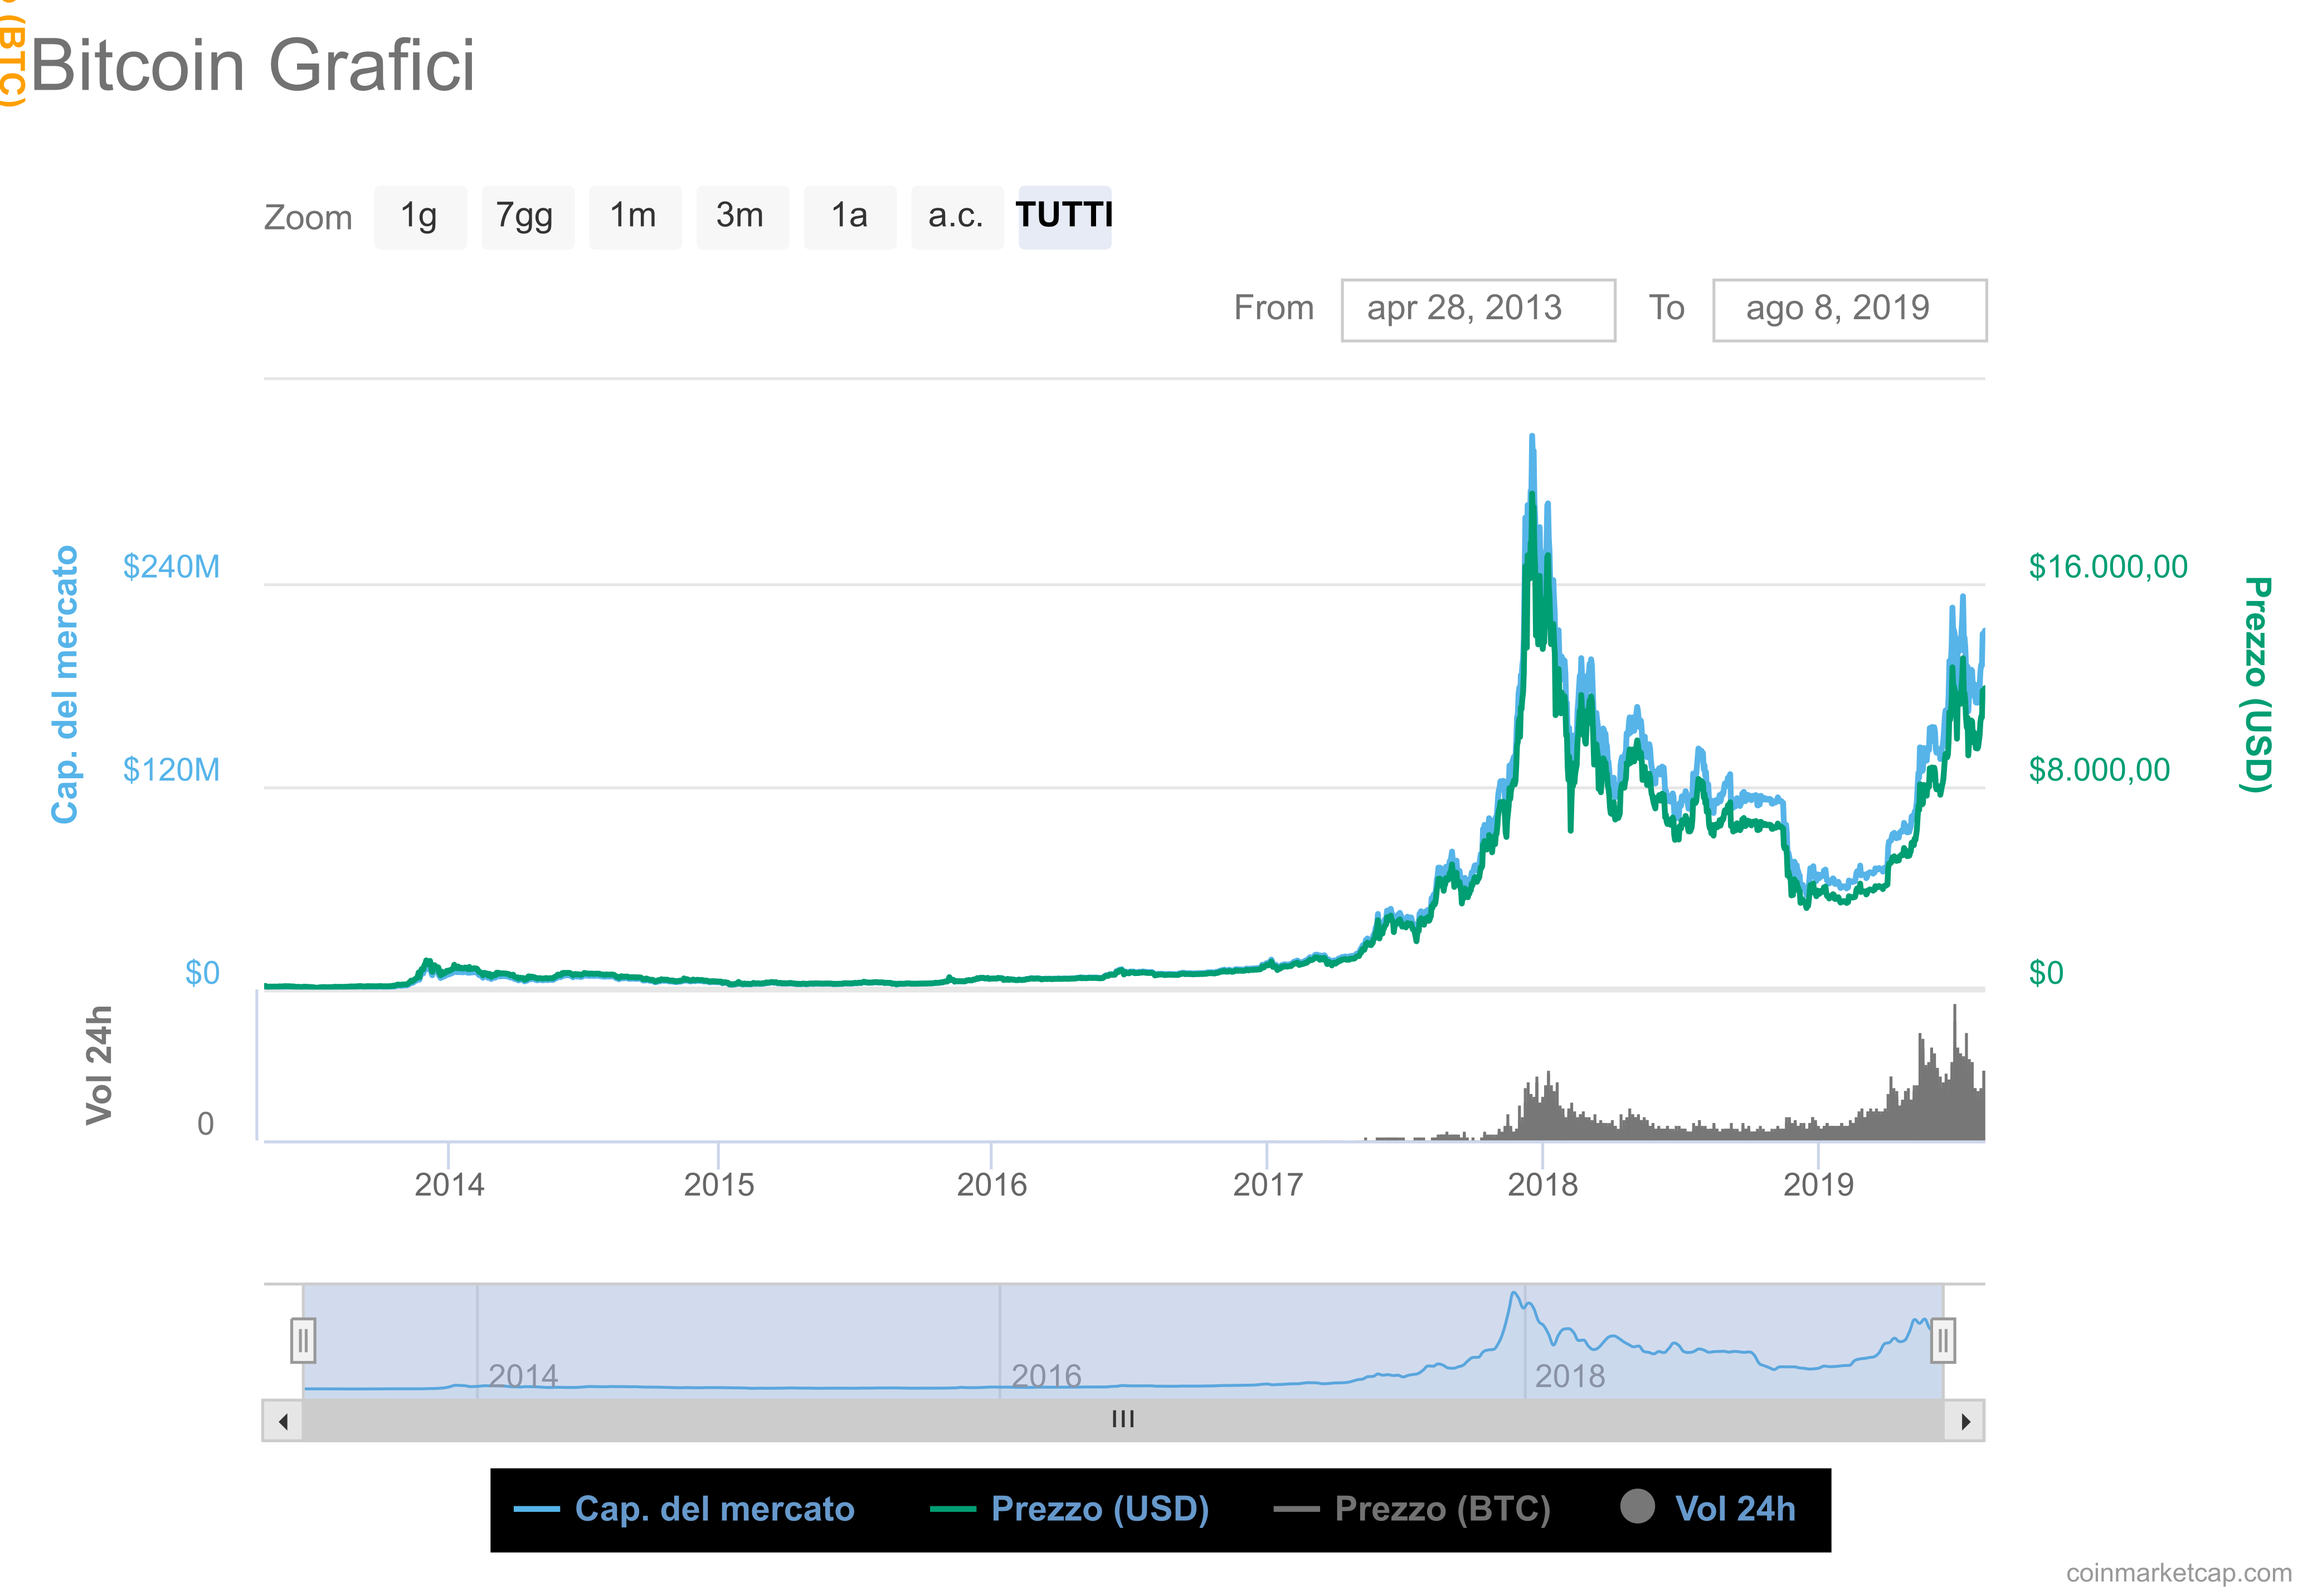
\includegraphics[width=\linewidth]{chartbitcoin.png}
  \caption{Bitcoin price chart}
  \label{fig:chartbitcoin}
\end{figure}


Ethereum viene descritto da Buterin in 

\section{Classificazione dei token nelle token sales}

\subsection{Il modello delle initial coin offering}
\subsection{Il modello delle security token offering}
